\documentclass[12pt,a4paper]{article}

% ─── Page Layout ───────────────────────────────────────────────────────────────
\usepackage[a4paper, margin=0.8in, headheight=14pt]{geometry}

% ─── Fonts (XeLaTeX) ───────────────────────────────────────────────────────────
\usepackage{fontspec}
\usepackage{unicode-math}
\setmainfont{TeX Gyre Pagella}
\setmonofont[Scale=0.88]{TeX Gyre Cursor}
\setmathfont{Latin Modern Math}

% ─── Packages ──────────────────────────────────────────────────────────────────
\usepackage{xcolor}
\usepackage{colortbl}
\usepackage{titlesec}
\usepackage{enumitem}
\usepackage{tabularx}
\usepackage{booktabs}
\usepackage{array}
\usepackage{amsmath}
\usepackage{tikz}
\usetikzlibrary{shapes.geometric, arrows.meta, positioning, calc, fit, decorations.pathreplacing}
\usepackage{tcolorbox}
\tcbuselibrary{skins, breakable}
\usepackage{hyperref}
\usepackage{fancyhdr}
\usepackage{graphicx}
\usepackage{microtype}
\hyphenpenalty=10000
\exhyphenpenalty=10000
\sloppy
\usepackage{caption}
\usepackage{setspace}
\usepackage{multirow}
\usepackage{tocloft}

% ─── Q&A helper ────────────────────────────────────────────────────────────────
\newcommand{\Q}[1]{\textbf{#1}\par\noindent\ignorespaces}

% ─── Colour Palette ────────────────────────────────────────────────────────────
\definecolor{myred}{RGB}{196,30,58}
\definecolor{mydark}{RGB}{30,30,50}
\definecolor{mygreen}{RGB}{14,120,80}
\definecolor{myteal}{RGB}{0,130,140}
\definecolor{myamber}{RGB}{180,100,0}
\definecolor{mypurple}{RGB}{100,30,160}
\definecolor{mygray}{RGB}{246,247,249}
\definecolor{mgframe}{RGB}{180,185,200}
\definecolor{watermark}{RGB}{145,150,170}
\definecolor{hdrred}{RGB}{250,232,235}
\definecolor{hdrgreen}{RGB}{220,244,233}
\definecolor{hdrteal}{RGB}{220,242,244}
\definecolor{hdramber}{RGB}{253,242,215}
\definecolor{hdrpurple}{RGB}{238,228,255}
\definecolor{hdrgray}{RGB}{238,240,245}
\definecolor{rowalt}{RGB}{250,251,253}

% ─── Section Formatting ────────────────────────────────────────────────────────
\titleformat{\section}
  {\large\bfseries\color{myred}}{\thesection.}{0.5em}{}
  [\vspace{1pt}{\color{myred}\rule{\linewidth}{0.8pt}}]
\titleformat{\subsection}
  {\normalsize\bfseries\color{myteal}}{\thesubsection}{0.5em}{}
\titlespacing*{\section}{0pt}{18pt}{7pt}
\titlespacing*{\subsection}{0pt}{11pt}{4pt}

% ─── Paragraph ─────────────────────────────────────────────────────────────────
\setlength{\parindent}{0pt}
\setlength{\parskip}{4pt}

% ─── TOC Styling ───────────────────────────────────────────────────────────────
\renewcommand{\cfttoctitlefont}{\large\bfseries\color{myred}}
\renewcommand{\cftaftertoctitle}{\par\noindent{\color{myred}\rule{\linewidth}{0.8pt}}}
\setlength{\cftbeforetoctitleskip}{0pt}
\setlength{\cftaftertoctitleskip}{6pt}
\renewcommand{\cftsecfont}{\normalsize\bfseries\color{mydark}}
\renewcommand{\cftsecpagefont}{\normalsize\bfseries\color{mydark}}
\renewcommand{\cftsecleader}{\cftdotfill{\cftdotsep}}
\setlength{\cftbeforesecskip}{7pt}
\renewcommand{\cftsubsecfont}{\small\color{mydark}}
\renewcommand{\cftsubsecpagefont}{\small\color{mydark}}
\setlength{\cftbeforesubsecskip}{3pt}
\setlength{\cftsubsecindent}{1.4em}

% ─── Table helpers ─────────────────────────────────────────────────────────────
\renewcommand{\arraystretch}{1.45}
\setlength{\tabcolsep}{6pt}
\arrayrulecolor{mydark}
\newcolumntype{B}[1]{>{\small\bfseries\raggedright\arraybackslash}m{#1}}
\newcolumntype{Y}{>{\small\raggedright\arraybackslash}X}
\renewcommand{\tabularxcolumn}[1]{m{#1}}

% ─── Header / Footer ───────────────────────────────────────────────────────────
\pagestyle{fancy}
\fancyhf{}
\fancyhead[L]{\small\color{myred}\textbf{EC501}\;\color{mydark}--- Electromagnetic Waves}
\fancyhead[R]{\small\color{myteal}\textbf{Module 4 Notes}}
\fancyfoot[C]{\small\color{mydark}\thepage}
\fancyfoot[R]{\small\color{watermark}\textit{\copyright\ Biraj}}
\renewcommand{\headrulewidth}{0.5pt}
\renewcommand{\footrulewidth}{0.3pt}

% ─── Hyperref ──────────────────────────────────────────────────────────────────
\hypersetup{
  colorlinks=true, linkcolor=myteal, urlcolor=myteal,
  pdfauthor={Biraj Sarkar},
  pdftitle={EC501 --- Module 4 Notes}
}

% ─── tcolorbox styles ──────────────────────────────────────────────────────────
\tcbset{
  tikzbox/.style={
    colback=mygray, colframe=mgframe, boxrule=0.6pt, arc=4pt,
    left=8pt, right=8pt, top=6pt, bottom=6pt,
    colbacktitle=mgframe, coltitle=mydark,
    fonttitle=\small\bfseries
  },
  defbox/.style={
    colback=hdrgreen, colframe=mygreen, boxrule=0.8pt, arc=4pt,
    left=9pt, right=9pt, top=6pt, bottom=6pt,
    colbacktitle=mygreen, coltitle=white,
    fonttitle=\small\bfseries
  },
  formulabox/.style={
    colback=hdrteal, colframe=myteal, boxrule=0.8pt, arc=4pt,
    left=9pt, right=9pt, top=7pt, bottom=7pt,
    colbacktitle=myteal, coltitle=white,
    fonttitle=\small\bfseries
  },
  examplebox/.style={
    colback=hdramber, colframe=myamber, boxrule=0.8pt, arc=4pt,
    left=9pt, right=9pt, top=6pt, bottom=6pt,
    colbacktitle=myamber, coltitle=white,
    fonttitle=\small\bfseries
  },
  masonbox/.style={
    colback=hdrpurple, colframe=mypurple, boxrule=0.8pt, arc=4pt,
    left=9pt, right=9pt, top=6pt, bottom=6pt,
    colbacktitle=mypurple, coltitle=white,
    fonttitle=\small\bfseries
  },
  exambox/.style={
    colback=hdrpurple, colframe=mypurple, boxrule=1pt, arc=5pt,
    left=10pt, right=10pt, top=8pt, bottom=8pt,
    colbacktitle=mypurple, coltitle=white,
    fonttitle=\bfseries,
    breakable, title after break={\textbf{Frequently Asked / Viva Questions (contd.)}}}
}
% Make all boxes breakable across pages
\tcbset{breakable}

% ─── TikZ styles ───────────────────────────────────────────────────────────────
\tikzset{
  block/.style={rectangle, draw=myteal, fill=hdrteal,
    text width=2.4cm, align=center, minimum height=0.95cm,
    font=\small, rounded corners=3pt, line width=0.7pt},
  redblock/.style={rectangle, draw=myred, fill=hdrred,
    text width=2.4cm, align=center, minimum height=0.95cm,
    font=\small, rounded corners=3pt, line width=0.7pt},
  netnode/.style={rectangle, draw=myteal, fill=hdrteal,
    text width=1.5cm, align=center, minimum height=0.8cm,
    font=\small, rounded corners=3pt, line width=0.7pt},
  sumjunc/.style={circle, draw=myamber, fill=hdramber,
    minimum size=0.62cm, font=\small, line width=0.8pt},
  snode/.style={circle, draw=mypurple, fill=hdrpurple,
    minimum size=0.55cm, font=\footnotesize, line width=0.7pt},
  arrow/.style={-Stealth, thick, color=mydark},
  redarrow/.style={-Stealth, thick, color=myred},
  line/.style={thick, color=mydark}
}

% ═══════════════════════════════════════════════════════════════════════════════
\begin{document}
% ═══════════════════════════════════════════════════════════════════════════════

\begin{center}
  {\LARGE\bfseries\color{myred} EC501 --- Electromagnetic Waves}\\[5pt]
  {\normalsize\color{mydark} Semester V \quad$\bullet$\quad 3L:0T:0P \quad$\bullet$\quad 3 Credits}\\[3pt]
  {\normalsize\color{myteal}\textbf{Module 4 Exam Notes: Parallel-Plate and Rectangular Waveguides}}\\[3pt]
  {\small\color{mydark} CGEC \;$|$\; B.Tech ECE (2023--27) \;$|$\; \textit{Biraj Sarkar}}
\end{center}
\vspace{2pt}
\noindent{\color{myred}\rule{\linewidth}{1.5pt}}
\vspace{2pt}

\hypersetup{linkcolor=mydark}
\tableofcontents
\hypersetup{linkcolor=myteal}
\newpage

\section{Waveguide Modes and the General Method}
\begin{tcolorbox}[defbox,title={Mode and cutoff}]
A mode is a field distribution that satisfies Maxwell's equations and the guide boundaries. Cutoff is the frequency separating propagating from evanescent behaviour for that mode in an ideal uniform guide.
\end{tcolorbox}

Assume a homogeneous lossless fill, perfect electric conductor (PEC) walls, $e^{j\omega t}$ and longitudinal dependence $e^{-j\beta z}$. Set $k=\omega\sqrt{\mu\epsilon}$ and let $\nabla_t$ act in the cross-section only.
\par\vspace{6pt}\noindent
\begin{tabularx}{\linewidth}{|B{2.5cm}|Y|Y|}\hline
Mode & Longitudinal fields & Boundary condition on the metal walls \\ \hline
TEM & $E_z=H_z=0$ & Transverse potential is constant on each conductor. \\ \hline
TE & $E_z=0,\ H_z\ne0$ & $\partial H_z/\partial n=0$ for the transverse normal. \\ \hline
TM & $H_z=0,\ E_z\ne0$ & $E_z=0$ at the wall. \\ \hline
\end{tabularx}
\subsection{Solve longitudinal fields first}
\begin{enumerate}[leftmargin=*,itemsep=4pt]
\item Separate the wave equation using $\partial_z=-j\beta$. Both longitudinal fields satisfy $(\nabla_t^2+k_c^2)\Psi=0$, where $k_c^2=k^2-\beta^2$.
\item Find allowed $k_c$ from the PEC conditions. TM uses a zero-value condition because $E_z$ is tangential to a longitudinal wall. For TE, tangential electric field is proportional to $\partial_n H_z$, giving a zero-derivative condition.
\item Recover transverse fields for $k_c\ne0$. In the transverse curl equations, substitute $\partial_z=-j\beta$ and eliminate $\mathbf H_t$ or $\mathbf E_t$ to get
\[
\begin{aligned}
\mathbf E_t
 &=-\frac{j\beta}{k_c^2}\nabla_tE_z
   +\frac{j\omega\mu}{k_c^2}\hat{\mathbf z}\times\nabla_tH_z,\\
\mathbf H_t
 &=-\frac{j\beta}{k_c^2}\nabla_tH_z
   -\frac{j\omega\epsilon}{k_c^2}\hat{\mathbf z}\times\nabla_tE_z .
\end{aligned}
\]
For example, in TE, Faraday's transverse equation gives $\mathbf H_t=(\beta/\omega\mu)\hat{\mathbf z}\times\mathbf E_t$. Substitution into transverse Amp\`ere--Maxwell yields $k_c^2\mathbf E_t=j\omega\mu\,\hat{\mathbf z}\times\nabla_tH_z$.
\item Test the frequency. Above cutoff $\beta=\sqrt{k^2-k_c^2}$ is real. Below cutoff choose $\beta=-j\sqrt{k_c^2-k^2}$ so the field decays along $+z$.
\end{enumerate}
\subsection{Cutoff, guide wavelength and velocity}
With $v=1/\sqrt{\mu\epsilon}$ and $f_c=vk_c/(2\pi)$, define $s=\sqrt{1-(f_c/f)^2}$ above cutoff.
\[
\beta=ks,\qquad\lambda_g=\frac{2\pi}{\beta}=\frac{\lambda}{s},\qquad
v_p=\frac{v}{s},\qquad v_g=vs .
\]
Differentiate $\beta^2=\omega^2/v^2-k_c^2$ to get $d\beta/d\omega=\omega/(\beta v^2)$. This yields $v_g=v^2/v_p$. The phase speed may exceed $v$ while the group speed stays below it. The wave impedances are ratios of transverse field components with the forward-power orientation:
\[
Z_{\mathrm{TE}}=\frac{\omega\mu}{\beta}=\frac{\eta}{s},
\qquad Z_{\mathrm{TM}}=\frac{\beta}{\omega\epsilon}=\eta s.
\]

\section{Parallel-Plate Waveguide}
\begin{tcolorbox}[defbox,title={Parallel-plate waveguide}]
Two parallel conducting plates guide waves along their length. In the ideal model the plates are at $y=0$ and $y=d$ with fields invariant in $x$.
\end{tcolorbox}
\begin{itemize}[leftmargin=*,itemsep=3pt]
\item \textbf{TEM.} Equipotential plates give a linear transverse potential and a uniform electric field normal to the plates. Choose $\mathbf E=E_0\hat{\mathbf y}e^{-jkz}$ and $\mathbf H=-(E_0/\eta)\hat{\mathbf x}e^{-jkz}$ for forward power. There is no cutoff. For width $w\gg d$ with negligible fringing, $Z_0$ for plate voltage and total current is $\eta d/w$, distinct from $E/H=\eta$.
\item \textbf{TE.} $\partial_y H_z=0$ at both plates, hence $H_z=H_0\cos(m\pi y/d)$ with $m=1,2,\ldots$. The constant candidate gives no TE field.
\item \textbf{TM.} $E_z=0$ at both plates, hence $E_z=E_0\sin(m\pi y/d)$ with $m=1,2,\ldots$.
\item \textbf{Modal propagation.} In both higher-mode families $k_c=m\pi/d$ and $f_c=mv/(2d)$. Between zero and the first cutoff only TEM propagates.
\end{itemize}
\begin{tcolorbox}[tikzbox,title={Parallel plates carrying a TEM wave},unbreakable]
\centering
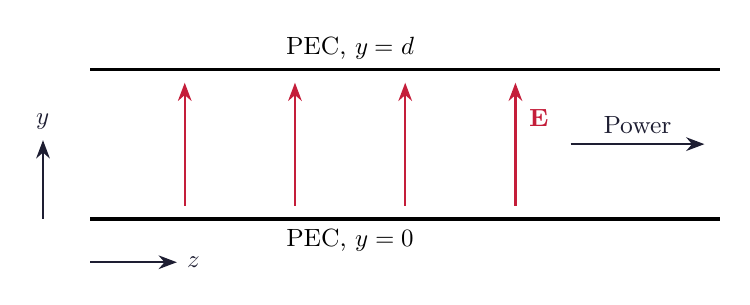
\begin{tikzpicture}[font=\small]
\draw[very thick] (0,0)--(8,0) (0,1.9)--(8,1.9);
\foreach \x in {1.2,2.6,4,5.4} \draw[redarrow] (\x,.17)--(\x,1.73);
\draw[arrow] (6.1,.95)--(7.8,.95) node[midway,above] {Power};
\draw[arrow] (0,-.55)--(1.1,-.55) node[right] {$z$};
\draw[arrow] (-.6,0)--(-.6,1) node[above] {$y$};
\node[above] at (3.3,1.9) {PEC, $y=d$};
\node[below] at (3.3,0) {PEC, $y=0$};
\node[right,myred] at (5.45,1.28) {$\mathbf E$};
\end{tikzpicture}
\end{tcolorbox}

\section{Rectangular Waveguide}
\subsection{Mode indices and dominant mode}
Let $a$ be the width in $x$ and $b$ the height in $y$. Separation in $x$ and $y$ gives $X''+k_x^2X=0$, $Y''+k_y^2Y=0$ and $k_x^2+k_y^2=k_c^2$. Enforcing the wall conditions gives
\[
\begin{aligned}
H_z&=H_0\cos(m\pi x/a)\cos(n\pi y/b)
 &&(\mathrm{TE},\ m,n\ge0,\ (m,n)\ne(0,0)),\\
E_z&=E_0\sin(m\pi x/a)\sin(n\pi y/b)
 &&(\mathrm{TM},\ m,n\ge1).
\end{aligned}
\]
Suppress the common $e^{-j\beta z}$ factor. Both families have
\[
 f_{c,mn}=\frac{v}{2}\sqrt{(m/a)^2+(n/b)^2}.
\]
For $a>b$, $\mathrm{TE}_{10}$ has the lowest cutoff $v/(2a)$ and is the dominant mode. The next cutoff is the smaller of $v/a$ ($\mathrm{TE}_{20}$) and $v/(2b)$ ($\mathrm{TE}_{01}$). Hollow single-conductor guide has no TEM mode. The transverse TEM potential would satisfy Laplace's equation with one constant value around the entire connected metal boundary. Uniqueness then forces a constant potential throughout and zero transverse electric field.
\subsection{Field visualization and surface current}
For $\mathrm{TE}_{10}$, let $k_x=\pi/a$ and drop the common axial factor. The only nonzero components are
\[
 H_z=H_0\cos(k_xx),\quad
 E_y=-\frac{j\omega\mu H_0}{k_x}\sin(k_xx),\quad
 H_x=\frac{j\beta H_0}{k_x}\sin(k_xx).
\]
At both side walls, tangential $E_y=0$ and $H_z$ is maximum in magnitude. Between these walls $|E_y|$ peaks at $a/2$. On the broad walls $E_y$ is normal, so its nonzero value is allowed and produces surface charge. There is no field variation across $y$ in this mode.
\begin{tcolorbox}[tikzbox,title={Electric field across the dominant-mode cross-section},unbreakable]
\centering
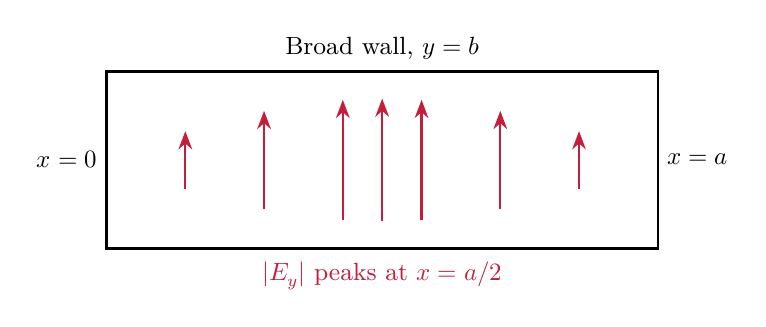
\begin{tikzpicture}[font=\small]
\draw[thick] (0,0) rectangle (7,2.25);
\foreach \x/\h in {1/.47,2/.8,3/.98,3.5/1,4/.98,5/.8,6/.47}
  \draw[redarrow] (\x,{1.125-.78*\h})--(\x,{1.125+.78*\h});
\node[above] at (3.5,2.28) {Broad wall, $y=b$};
\node[left] at (0,1.13) {$x=0$};
\node[right] at (7,1.13) {$x=a$};
\node[below,myred] at (3.5,-.04) {$|E_y|$ peaks at $x=a/2$};
\end{tikzpicture}
\end{tcolorbox}

For wall current, use the normal pointing from metal into guide and $\mathbf K=\hat{\mathbf n}\times\mathbf H$. At $x=0$, $\hat{\mathbf n}=\hat{\mathbf x}$ and $\mathbf K=-H_z\hat{\mathbf y}$. At $x=a$, $\hat{\mathbf n}=-\hat{\mathbf x}$ and $H_z=-H_0$, so $\mathbf K$ again points along $-\hat{\mathbf y}$ for the same $H_0$ phase. On the broad walls, the normal is $\pm\hat{\mathbf y}$. The wall current has both $x$ and $z$ components from $H_z$ and $H_x$, respectively. The current flows tangentially on all walls.

\subsection{Higher-mode field sketch and coupling}
For $\mathrm{TE}_{11}$ write $k_x=\pi/a$, $k_y=\pi/b$, $k_c^2=k_x^2+k_y^2$ and $H_z=H_0\cos(k_xx)\cos(k_yy)$. Use the TE transverse-field relation to get
\[
\begin{aligned}
 E_x &= \frac{j\omega\mu H_0 k_y}{k_c^2}\cos(k_xx)\sin(k_yy),\\
 E_y &=-\frac{j\omega\mu H_0 k_x}{k_c^2}\sin(k_xx)\cos(k_yy).
\end{aligned}
\]
To sketch, mark the midlines $x=a/2$ and $y=b/2$. On the $y$ midline only $E_x$ remains. On the $x$ midline only $E_y$ remains. All tangential electric components vanish at the PEC wall. Both components vanish at the centre of this particular mode.
\begin{tcolorbox}[tikzbox,title={TE11 cross-section at one field phase},unbreakable]
\centering
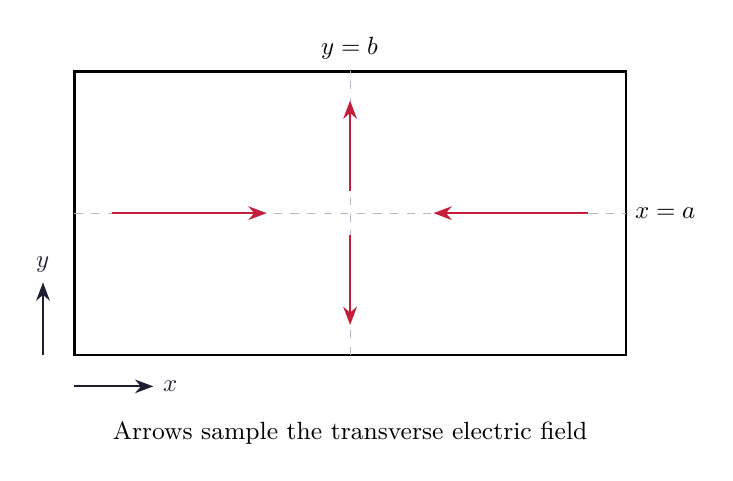
\begin{tikzpicture}[font=\small]
\draw[thick] (0,0) rectangle (7,3.6);
\draw[dashed,mgframe] (3.5,0)--(3.5,3.6) (0,1.8)--(7,1.8);
\draw[redarrow] (.48,1.8)--(2.44,1.8);
\draw[redarrow] (6.52,1.8)--(4.56,1.8);
\draw[redarrow] (3.5,1.52)--(3.5,.38);
\draw[redarrow] (3.5,2.08)--(3.5,3.23);
\draw[arrow] (0,-.4)--(1,-.4) node[right] {$x$};
\draw[arrow] (-.4,0)--(-.4,.92) node[above] {$y$};
\node[above] at (3.5,3.63) {$y=b$};
\node[right] at (7,1.8) {$x=a$};
\node[below] at (3.5,-.72) {Arrows sample the transverse electric field};
\end{tikzpicture}
\end{tcolorbox}

\textbf{Coupling out power.} An electric probe couples when it is placed at a nonzero electric field and aligned with that field. For example, a small $y$-directed probe at $x=a/2$, $y=b/4$ samples $E_y$ in $\mathrm{TE}_{11}$. A small loop instead couples to magnetic flux when its normal is aligned with the local magnetic field. Coupling also depends on which other modes are above cutoff and on how the coupler is matched.

\begin{tcolorbox}[examplebox,title={Cutoff ordering and below-cutoff decay}]
An air-filled guide has $a=30\,\mathrm{mm}$ and $b=15\,\mathrm{mm}$. The $\mathrm{TE}_{10}$ cutoff is $5\,\mathrm{GHz}$ and the $\mathrm{TE}_{20}$ and $\mathrm{TE}_{01}$ cutoffs are both $10\,\mathrm{GHz}$. The $\mathrm{TE}_{11}$ and $\mathrm{TM}_{11}$ cutoffs are both $\sqrt{5^2+10^2}=11.18\,\mathrm{GHz}$.

At $8\,\mathrm{GHz}$, only $\mathrm{TE}_{10}$ propagates. A semi-infinite guide's below-cutoff $\mathrm{TE}_{11}$ component decays with constant $\kappa=(2\pi/v)\sqrt{f_c^2-f^2}\approx164\,\mathrm{m^{-1}}$. At $20\,\mathrm{mm}$ the amplitude fraction is $e^{-\kappa(0.020)}\approx0.038$. This cutoff decay exists even with perfect walls. Ohmic attenuation above cutoff is a separate effect.
\end{tcolorbox}

\section{Guide Attenuation and Numerical Design}
\begin{tcolorbox}[defbox,title={Attenuation constant}]
If amplitude varies as $e^{-\alpha z}$, guided power varies as $e^{-2\alpha z}$. The amplitude attenuation is $\alpha$ in nepers per metre, or $8.686\alpha$ in decibels per metre.
\end{tcolorbox}
\begin{enumerate}[leftmargin=*,itemsep=4pt]
\item \textbf{Calculate transmitted power.} Use the ideal modal fields for small loss: $P=\tfrac12\operatorname{Re}\int_A(\mathbf E\times\mathbf H^*)\cdot\hat{\mathbf z}\,dA$.
\item \textbf{Calculate wall loss per metre.} The surface resistance is $R_s=\sqrt{\omega\mu_w/(2\sigma_w)}$ for a good metal. Integrate $P'_w=(R_s/2)\oint |\mathbf H_{\tan}|^2\,ds$ around the perimeter. Include both pairs of walls.
\item \textbf{Convert loss to attenuation.} Power balance gives $-dP/dz=P'_w=2\alpha_cP$, so $\alpha_c=P'_w/(2P)$.
\end{enumerate}
For $\mathrm{TE}_{10}$, integration of $\sin^2(k_xx)$ gives $a/2$. Thus $P=ab\,\omega\mu\beta |H_0|^2/(4k_x^2)$. The two side walls contribute $2b|H_0|^2$ to the perimeter integral. The broad walls contribute $a(1+\beta^2/k_x^2)|H_0|^2$. Substituting and using $q=f_c/f=k_x/k$ yields
\[
\alpha_c=\frac{R_s}{\eta b\sqrt{1-q^2}}\left[1+\frac{2b}{a}q^2\right].
\]
For a weakly lossy dielectric with loss tangent $\tan\delta_d$, replace $k^2$ by $k^2(1-j\tan\delta_d)$. Expanding the square root yields $\alpha_d\approx k^2\tan\delta_d/(2\beta)$. Add the two contributions when losses are small. Near cutoff, these perturbative estimates lose accuracy as $\beta\to0$.
\begin{tcolorbox}[examplebox,title={Single-mode test at 10 GHz}]
Take an air-filled guide $a=22.86\,\mathrm{mm}$, $b=10.16\,\mathrm{mm}$.
\begin{enumerate}[leftmargin=*,itemsep=2pt]
\item $f_{c,10}=6.56\,\mathrm{GHz}$, $f_{c,20}=13.12\,\mathrm{GHz}$, $f_{c,01}=14.76\,\mathrm{GHz}$. Only $\mathrm{TE}_{10}$ propagates at $10\,\mathrm{GHz}$.
\item With $\lambda=30.0\,\mathrm{mm}$ and $s=0.755$, $\lambda_g=39.7\,\mathrm{mm}$, $v_g=2.26\times10^8\,\mathrm{m/s}$ and $Z_{\mathrm{TE}}\approx499\,\Omega$.
\item For smooth copper with $R_s\approx0.0261\,\Omega$, $\alpha_c\approx0.0125\,\mathrm{Np/m}\approx0.109\,\mathrm{dB/m}$. Ideal air adds negligible dielectric loss.
\end{enumerate}
\end{tcolorbox}

\newpage
\begin{center}
  {\large\bfseries\color{myred} Quick Revision --- Module 4}\\[3pt]
  {\small\color{mydark} Parallel-Plate and Rectangular Waveguides $|$ EC501}
\end{center}
\noindent{\color{myred}\rule{\linewidth}{1.2pt}}
\begin{tcolorbox}[formulabox,title={Key Formulas at a Glance}]
\renewcommand{\arraystretch}{1.35}
\begin{tabularx}{\linewidth}{B{5.0cm}Y}
Dispersion relation & $\beta^2=k^2-k_c^2$ \\[3pt]
Plate cutoff & $f_c=mv/(2d)$ for higher modes \\[3pt]
Rectangular cutoff & $f_{c,mn}=(v/2)\sqrt{(m/a)^2+(n/b)^2}$ \\[3pt]
Guide wavelength & $\lambda_g=2\pi/\beta$ \\[3pt]
Wall current & $\mathbf K=\hat{\mathbf n}\times\mathbf H$ with metal-to-guide normal \\[3pt]
Amplitude attenuation & $\alpha_c=P'_w/(2P)$ \\[3pt]
\end{tabularx}
\end{tcolorbox}
\begin{tcolorbox}[defbox,title={One-Line Definitions}]
\textbf{Dominant mode.} Mode with the lowest cutoff frequency.\par
\textbf{Guide wavelength.} Distance along the guide giving a phase advance of one full cycle.\par
\textbf{Below-cutoff field.} Evanescent field that decays along the guide in a semi-infinite section.\par
\end{tcolorbox}
\begin{tcolorbox}[exambox,title={Frequently Asked / Viva Questions}]
\begin{enumerate}[topsep=0pt, label=\textbf{Q\arabic*.}, itemsep=5pt]
\item \Q{Why does a parallel-plate guide support TEM?}
Distinct conductors can be held at different transverse potentials.
\item \Q{Why does hollow rectangular guide lack TEM?}
Its single connected metal boundary forces a constant transverse potential.
\item \Q{Why can TE have one zero index?}
Cosine remains nonzero when one transverse index is zero.
\item \Q{Why cannot TM have a zero index?}
Its sine product vanishes identically.
\item \Q{What is dominant when the width exceeds the height?}
The $\mathrm{TE}_{10}$ mode.
\item \Q{What determines single-mode operation?}
Frequency lies above dominant cutoff and below the next allowed cutoff.
\item \Q{How do phase and group velocity compare?}
Above cutoff their product is $v^2$ for a nondispersive fill and ideal walls.
\item \Q{Where is the dominant-mode electric field largest?}
At $x=a/2$, directed across the guide height.
\item \Q{Which magnetic field determines wall loss?}
The field tangential to the metal.
\item \Q{Why is attenuation generally larger near cutoff?}
Modal power for a given field level drops as $\beta$ falls.
\end{enumerate}
\end{tcolorbox}
\begin{tcolorbox}[tikzbox,title={Summary comparison}]
\begin{tabularx}{\linewidth}{|B{4cm}|Y|}\hline
\textbf{Case} & \textbf{What to use} \\ \hline
TEM parallel plates & No cutoff. Both longitudinal components vanish. \\ \hline
TE rectangular & $H_z$ cosine product. One index may be zero. \\ \hline
TM rectangular & $E_z$ sine product. Both indices must be positive. \\ \hline
\end{tabularx}
\end{tcolorbox}
\end{document}
